\chapter{Introduction}
\label{chap:intro}

%%%%%%%%%%%%%%%%%%%%%%%%%%%%%%%%%%%%%%%%%%%%%%%%%%%%%%%%%%%%%%%%%%%%%%%%%%%%%%%
\section{Background}
\label{sec:chap1-background}


\begin{figure}
\begin{subfigure}{.5\textwidth}
  \centering
  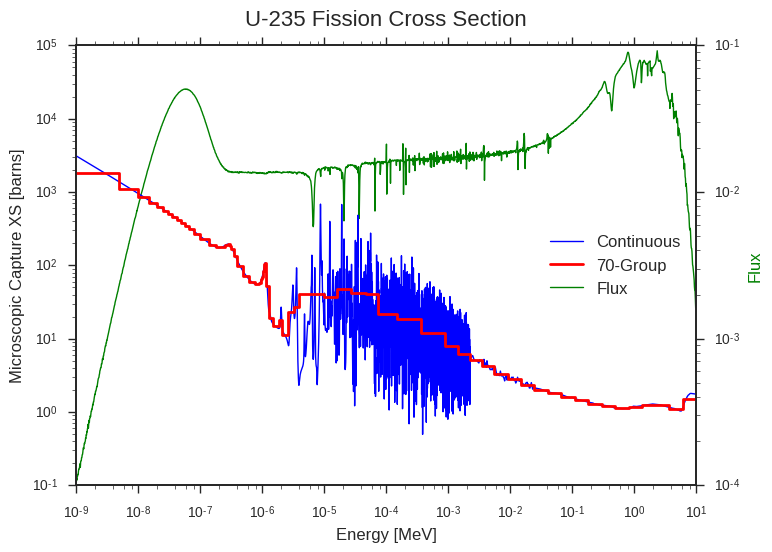
\includegraphics[width=\linewidth]{figures/intro/u235-fission-70}
  \caption{}
  \label{fig:assm-cells}
\end{subfigure}%
\begin{subfigure}{.5\textwidth}
  \centering
  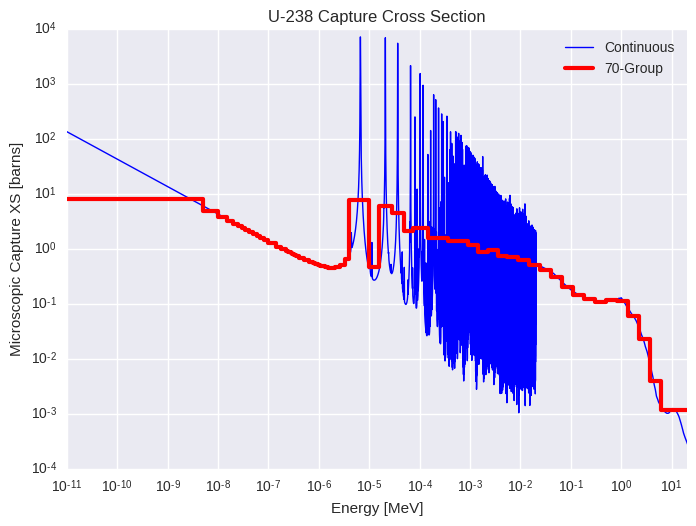
\includegraphics[width=\linewidth]{figures/intro/u238-capture-70}
  \caption{}
  \label{fig:colorset-cells}
\end{subfigure}
\begin{subfigure}{.5\textwidth}
  \centering
  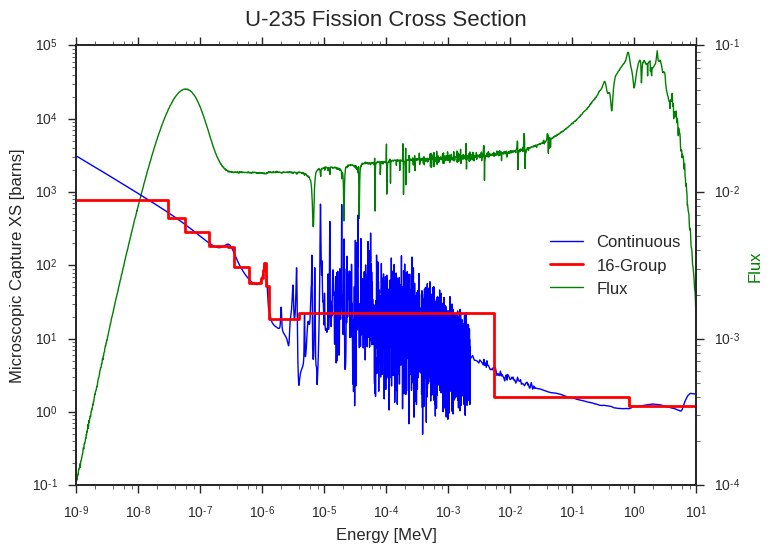
\includegraphics[width=\linewidth]{figures/intro/u235-fission-16}
  \caption{}
  \label{fig:assm-unique-neighbors}
\end{subfigure}
\begin{subfigure}{.5\textwidth}
  \centering
  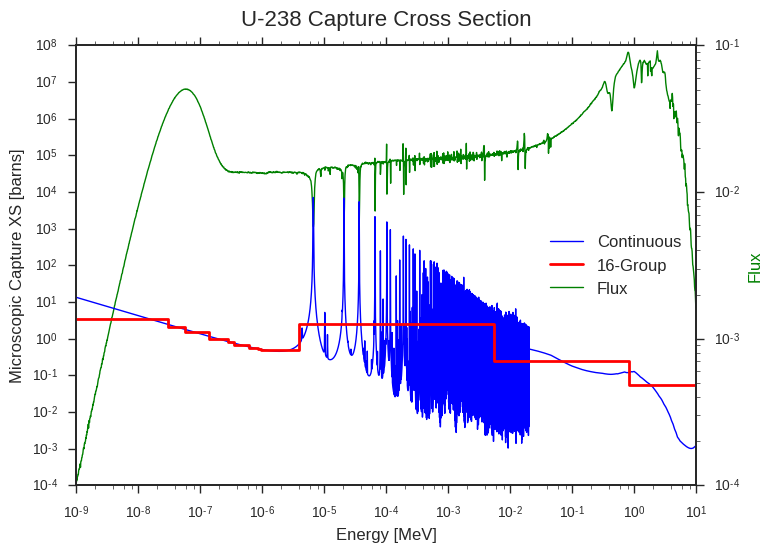
\includegraphics[width=\linewidth]{figures/intro/u238-capture-16}
  \caption{}
  \label{fig:colorset-unique-neighbors}
\end{subfigure}
\begin{subfigure}{.5\textwidth}
  \centering
  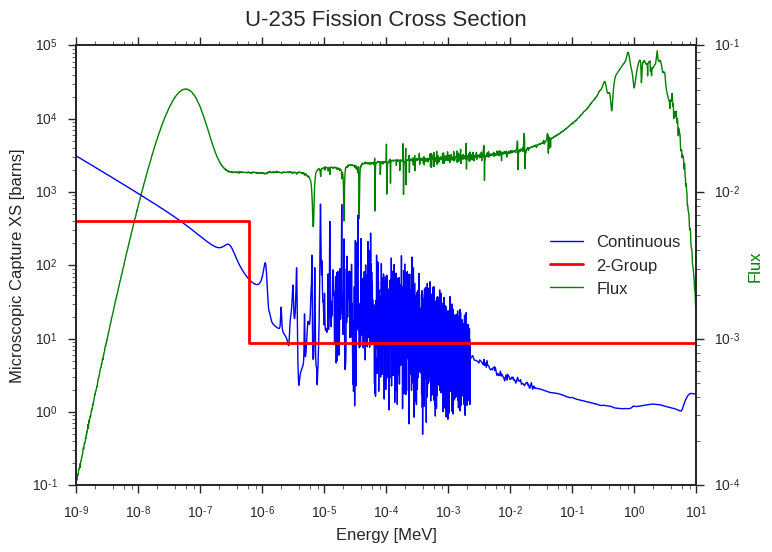
\includegraphics[width=\linewidth]{figures/intro/u235-fission-2}
  \caption{}
  \label{fig:assm-neighbors}
\end{subfigure}
\begin{subfigure}{.5\textwidth}
  \centering
  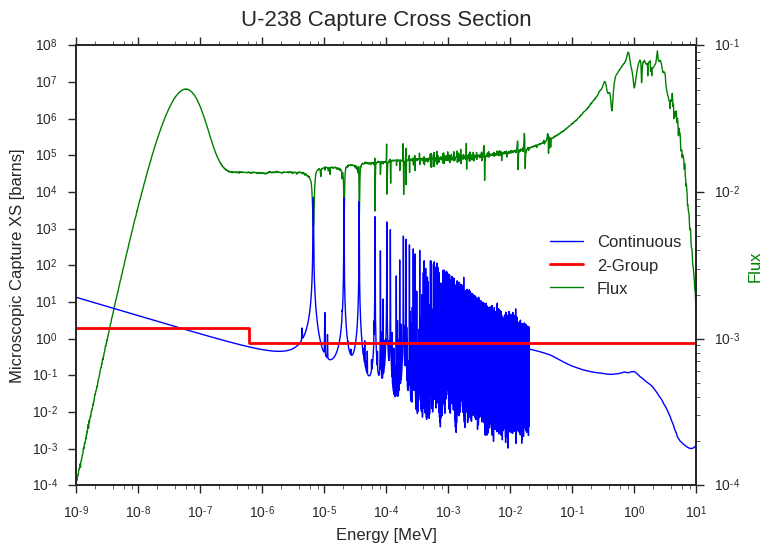
\includegraphics[width=\linewidth]{figures/intro/u238-capture-2}
  \caption{}
  \label{fig:colorset-neighbors}
\end{subfigure}
\caption[Uranium-235 and Uranium-238 cross sections]{Continuous energy and multi-group cross sections for U-235 fission (left) and U-238 capture (right) reactions in a PWR spectrum for 70-, 16- and 2-groups.}
\label{fig:pwr-ce-mg-xs}
\end{figure}


%%%%%%%%%%%%%%%%%%%%%%%%%%%%%%%%%%%%%%%%%%%%%%%%%%%%%%%%%%%%%%%%%%%%%%%%%%%%%%%
\section{High-Performance Computing Trends}
\label{sec:chap1-hpc-trends}

\cite{Hunter_Sutton_2013}


%%%%%%%%%%%%%%%%%%%%%%%%%%%%%%%%%%%%%%%%%%%%%%%%%%%%%%%%%%%%%%%%%%%%%%%%%%%%%%%
\section{Whole-Core Neutron Transport Simulations}
\label{sec:chap1-whole-core-transport}

\begin{dmath}
\label{eqn:chap1-transport-eqn-6d}
\mathbf{\Omega} \cdot \nabla \Psi(\mathbf{r},\mathbf{\Omega},E) + \Sigma^T(\mathbf{r},E)\Psi(\mathbf{r},\mathbf{\Omega},E) = \int_{0}^{\infty} \mathrm{d}E' \int_{4\pi} \mathrm{d}\mathbf{\Omega'}\Sigma^S(\mathbf{r},{\mathbf{\Omega'}\rightarrow\mathbf{\Omega}},{E'\rightarrow E}) \Psi(\mathbf{r},\mathbf{\Omega'},E') + \frac{\chi(\mathbf{r},E)}{4\pi k_{eff}} \int_{0}^{\infty} \mathrm{d}E' \nu\Sigma^F(\mathbf{r},E') \int_{4\pi} \mathrm{d}\mathbf{\Omega'}\Psi(\mathbf{r},\mathbf{\Omega'},E')
\end{dmath}

Each of the variables in use is defined in \autoref{tab:moc-variables}. This is a balance equation between neutrons lost to transport, lost to absorption, produced or lost from scattering and those produced from fission. It should be noted that this equation assumes isotropic emission from fission.

\begin{table}[hbt]
  \caption{Variables in the Boltzmann equation.}
  \label{tab:chap1-variables}
  \begin{center}
    \begin{tabular}{ l l }
    \toprule
    Variable & Description \\
    \midrule
    $\mathbf{r}$ & Spatial position vector \\
    $\mathbf{\Omega}$ & Angular direction vector \\
    $E$ & Neutron energy \\
    $\Psi$ & Angular neutron flux \\
    $k_{eff}$ & Effective neutron multiplication factor \\
    $\Sigma^T$ & Neutron total cross-section \\
    $\Sigma^S$ & Neutron scattering cross-section \\
    $\Sigma^F$ & Neutron fission cross-section \\
    $\chi$ & Energy spectrum for fission neutrons \\
    $\nu$ & Average number of neutrons emitted per fission \\
    \bottomrule
  \end{tabular}
  \end{center}
\end{table}


%%%%%%%%%%%%%%%%%%%%%%%%%%%%%%%%
\subsection{Monte Carlo Methods}
\label{subsec:chap1-monte-carlo}


%%%%%%%%%%%%%%%%%%%%%%%%%%%%%%%%%%
\subsection{Deterministic Methods}
\label{subsec:chap1-deterministic}

\begin{itemize}
  \item 2D/1D methods in MPACT, nTracer
  \item Denovo, PDT, 3D OpenMOC, etc.
\end{itemize}


%%%%%%%%%%%%%%%%%%%%%%%%%%%%%%%%%%%%%%%%%%%%%%%%%%%%%%%%%%%%%%%%%%%%%%%%%%%%%%%
\section{Multi-Group Cross Sections}
\label{sec:chap1-mgxs}

\begin{itemize}[noitemsep]
  \item black magic ``crux'' of deterministic methods
  \item need accurate \ac{MGXS} for whole core transport methods
  \item motivate \ac{MC} for \ac{MGXS}
\end{itemize}